\chapter*{Einführung in das GeomInt-Vorhaben}
\label{cha:geomint-de}

\Authors{Thomas Nagel, Uwe-Jens G\"orke, Heinz Konietzky, Jobst Ma{\ss}mann, Mathias Nest, Holger Steeb, Frank Wuttke, Olaf Kolditz}

\section*{Hintergrund} 

Die Nutzung des untertägigen Raumes als Ressourcenquelle, Speicher und Verkehrsraum ist in den vergangenen Jahren deutlich intensiver und vielfältiger geworden. Neben klassischen anthropogenen Eingriffen wie Bergbau, Förderung von Erdöl und Erdgas oder Tunnelbau sind besonders im Zusammenhang mit Fragen der Transformation von Energiesystemen weitere Nutzungsformen des untertägigen Raumes in den Blickpunkt wirtschaftlicher, politischer und wissenschaftlicher Untersuchungen geraten. Dazu gehören beispielsweise die Gewinnung von Energie (z. B. Geothermie) und Energieträgern unter Einsatz neuer Technologien (z.B. unkonventionelle Gasgewinnung) sowie die geologische Kurz- und Langzeitspeicherung von Energieträgern (z.B. Druckluft, Wasserstoff, Methan) und die sichere Verwahrung von Abfällen, die bei der Energieproduktion oder in anderen Industriebereichen anfallen (z.B. Kohlendioxid, radioaktive Abfälle).

Zunehmende Eingriffe in den geologischen Untergrund erfordern sorgfältige Zustandsanalysen der Gesteins-Fluid-Systeme sowie Bewertungen zu Machbarkeit, Effizienz und Umweltauswirkungen der betrachteten Technologien. Die Einrichtung eines wirtschaftlichen und ökologischen Betriebs sowie der Sicherheit von untertägigen Geosystemen erfordern das umfassende Verständnis der physikalischen, (geo)chemischen und mikrobiologischen Prozesse auf allen relevanten Zeit- und Längenskalen. Dieses Verständnis kann nur auf der Basis intensiver Labor- und In-situ-Experimente im Zusammenhang mit zuverlässigen Studien zur Modellierung und Simulation (numerisches Experiment) der entsprechenden Prozesse vertieft werden.

Die Festgesteine des untertägigen Raumes zeichnen sich durch ein komplexes Materialverhalten aus. Unter realen Belastungsbedingungen treten irreversible Verformungen, geschwindigkeitsabhängiges Festigkeitsverhalten sowie Kriech-, Quell- und Schrumpfeffekte auf.

Dämpfungsaspekte, beispielsweise im Bereich niederfrequenter seismischer Wellen, Schädigung und physikalisch-chemische Alterung (z. B. Lösungs- und/oder Fällungsreaktionen) spielen in vielen geophysikalischen Fragestellungen eine bedeutende Rolle. Insbesondere die Themen Schädigung, Rissbildung und -ausbreitung sowie Grenzflächenproblematik sind Aspekte, die einer weiteren Klärung bedürfen.  Aufgrund der in diesen Bereichen vorherrschenden Wissenslücken können viele solcher Prozesse derzeit mit kommerziellen numerischen Simulationssystemen, die üblicherweise in der geotechnischen Praxis verwendet werden, nicht angemessen modelliert werden. Sie stellen daher Themen dar, die dringend erforscht werden müssen. Die entsprechenden Prozesse manifestieren sich in verschiedenen mikro- und makromechanischen Verhaltensstrukturen der betrachteten Materialien und werden hier unter dem Oberbegriff Diskontinuitäten zusammengefasst (Abb. ~\ref{fig:pro01}).

%\begin{figure}[ht!]
%\centering
%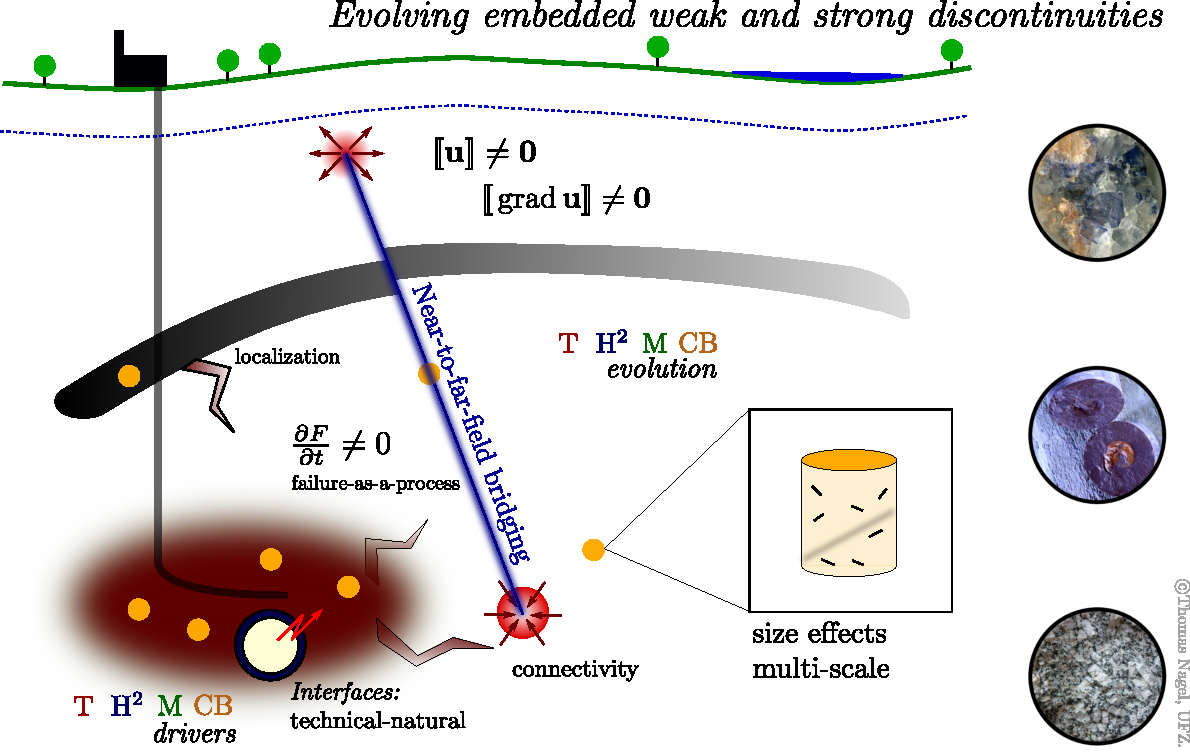
\includegraphics[width=1\textwidth]{figures/Barrier_concept.pdf}
%\caption{Grafische Übersicht zum GeomInt-Projekt mit Darstellung des grundlegenden Konzepts bezüglich der Diskontinuitäten Prozesse in verschiedenen Gesteinsarten}
%\label{fig:pro01-de}
%\end{figure}

\section*{Das GeomInt-Projekt}
\label{sec:geomint-de}

GeomInt (Geomechanische Integrität von Wirts- und Barrieregesteinen - Experiment, Modellierung und Analyse von Diskontinuitäten) trägt zur realistischen und anwendungsorientierten experimentell-numerischen Analyse der Entstehung und Entwicklung von Diskontinuitäten in den untertägigen Gesteinen Steinsalze, Tongesteine und Kristallingesteine bei. Im Folgenden werden diese Gesteine auch kurz als Salz, Ton und Kristallin bezeichnet. Das Verständnis und die Quantifizierung von Wechselwirkungen mit sich dynamisch entwickelnden Gesteinseigenschaften (z. B. Permeabilität), welche die geomechanische Integrität und Dichtheit geologischer Reservoir-Barriere-Systeme bestimmen, stehen dabei im Mittelpunkt. In die Untersuchungen einbezogen sind Diskontinuitäten volumetrisch verteilter Schädigungen, wie sie in der Auflockerungszone von Festgesteinen auftreten, Diskontinuitäten, die sich an Phasengrenzflächen unkontrolliert oder kontrolliert bilden können, sowie diskrete Riss- und Kluftnetzwerke. Die durch diese Diskontinuitäten geschaffenen bzw. erweiterten Wegsamkeiten für Fluide in Wirts- und Barrieregesteinen bergen das Risiko, dass, beispielsweise durch die Migration fluider Phasen aus tiefen in oberflächennahe geologische Schichten und letztendlich bis in die Biosphäre, lebenswichtige Ökosysteme nachhaltig beeinträchtigt werden können. Eine Reihe von thermisch-hydraulisch-mechanisch-chemisch (THMC) gekoppelten Prozessen kann zur Entwicklung von Diskontinuitäten im Nahfeld einer geotechnischen Infrastruktur führen, was wiederum die Generierung zuvor nicht vorhandener Konnektivitäten führt. Wenn dabei eine Verbindung zu leitfähigen Bruchzonen oder Kluftnetzwerken mit einer bestimmten Reichweite hergestellt wird, kann der Transport in das Fernfeld in einem viel kürzeren Zeitrahmen als zuvor möglich werden (Abb. ~\ref{fig:pro01}).

%\begin{figure}[ht!]
%\begin{minipage}{0.69\textwidth}
%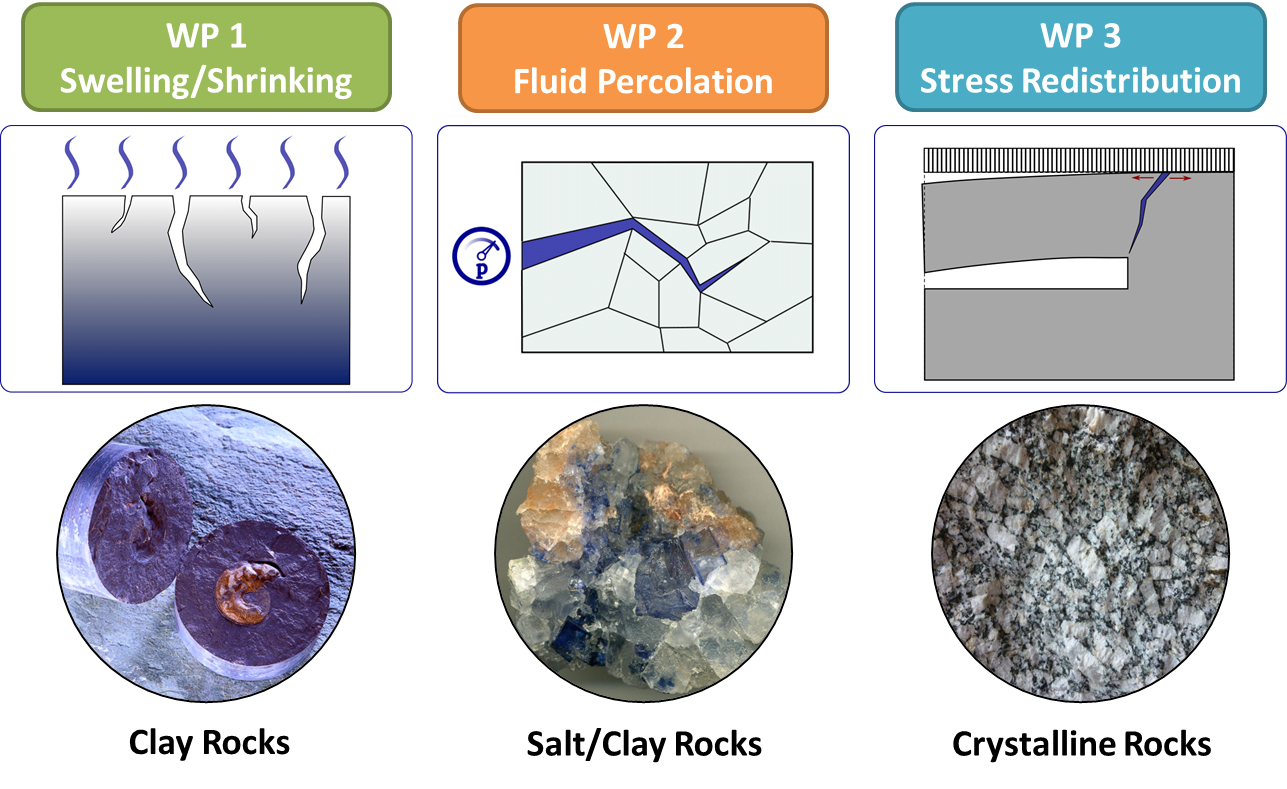
\includegraphics[width=1\textwidth]{figures/geomint-concept-02.png}
%\end{minipage}
%\hfill
%\begin{minipage}{0.29\textwidth}
%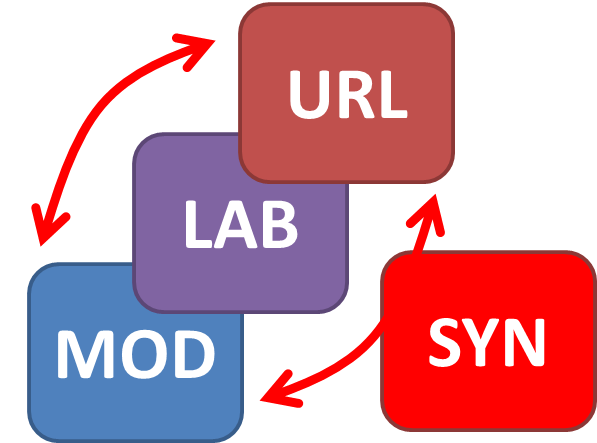
\includegraphics[width=1\textwidth]{figures/modal01a.png}
%\end{minipage}
%\caption{Arbeitspaketstruktur von GeomInt und Kombination von experimentellen und Modellierungsarbeiten: Hauptmechanismen für die Entwicklung und Ausbreitung von Diskontinuitäten in verschiedenen Gesteinsarten}
%\label{fig:pro02-de}
%\end{figure}

GeomInt wird von einem interdisziplinären Konsortium aus Partnern von Universitäten, staatlichen und privaten Forschungseinrichtungen mit sich ergänzenden, langjährigen Erfahrungen in der Analyse untertägiger Geosysteme bearbeitet. Drei typische Effekte, die zur Entstehung und Entwicklung spezifischer Diskontinuitäten führen, werden als Forschungsschwerpunkte betrachtet: Quell- und Schrumpfungsprozesse, druckgetrieben Perkolation und Spannungsumlagerungen (Abb.~\ref{fig:pro02}). 
Die Forschungsarbeiten sind dabei jeweils in die Bereiche Laborexperiment, numerische Simulationen und In-situ-Experimente (Untertagelabore – URLs) strukturiert. Von den Laborexperimenten wurden neue Erkenntnisse zum Prozessverständnis gewonnen. Insbesondere wurden Beiträge gekoppelter thermischer, hydraulischer und mechanischer Prozesse für die Bildung und Entwicklung von Diskontinuitäten berücksichtigt. Diese Erkenntnisse wurden verwendet, um die Weiterentwicklung verschiedener kontinuumsmechanischer, diskontinuumsmechanischer und hybrider numerischer Ansätze zu unterstützen und deren Potenziale und Limitierungen zu vergleichen. Neuartige Modelle und Algorithmen wurden hauptsächlich in wissenschaftliche Software implementiert, die der Forschungslandschaft zur Verfügung steht. Die Eignung der Modelle für die Analyse und Prognose realistischer Betriebsszenarien untertägiger Geosysteme (z.B. geothermische Reservoire, geologische Speicher für Energieträger und Abfälle) wird anhand von Testfeldsimulationen verschiedener In-situ Experimente weiter validiert und wurde hauptsächlich unter Nutzung von Synergien mit anderen nationalen und internationalen Forschungsvorhaben in Untertagelaboren durchgeführt, die den Projektpartnern von GeomInt zugänglich sind.

Die fachwissenschaftlichen Arbeitspakete des Vorhabens wurden mit Syntheseaktivitäten wie Daten- und Modellintegration unter Verwendung von VR-Methoden (Virtual Reality) verknüpft (Abb.~\ref{fig:pro03}).
Ein entsprechender Pilotdemonstrator wurde für das Mont Terri-Projekt implementiert (Abb. ~\ref{fig:pro03}, rechts).

%\begin{figure}[ht!]
%\begin{minipage}{0.49\textwidth}
%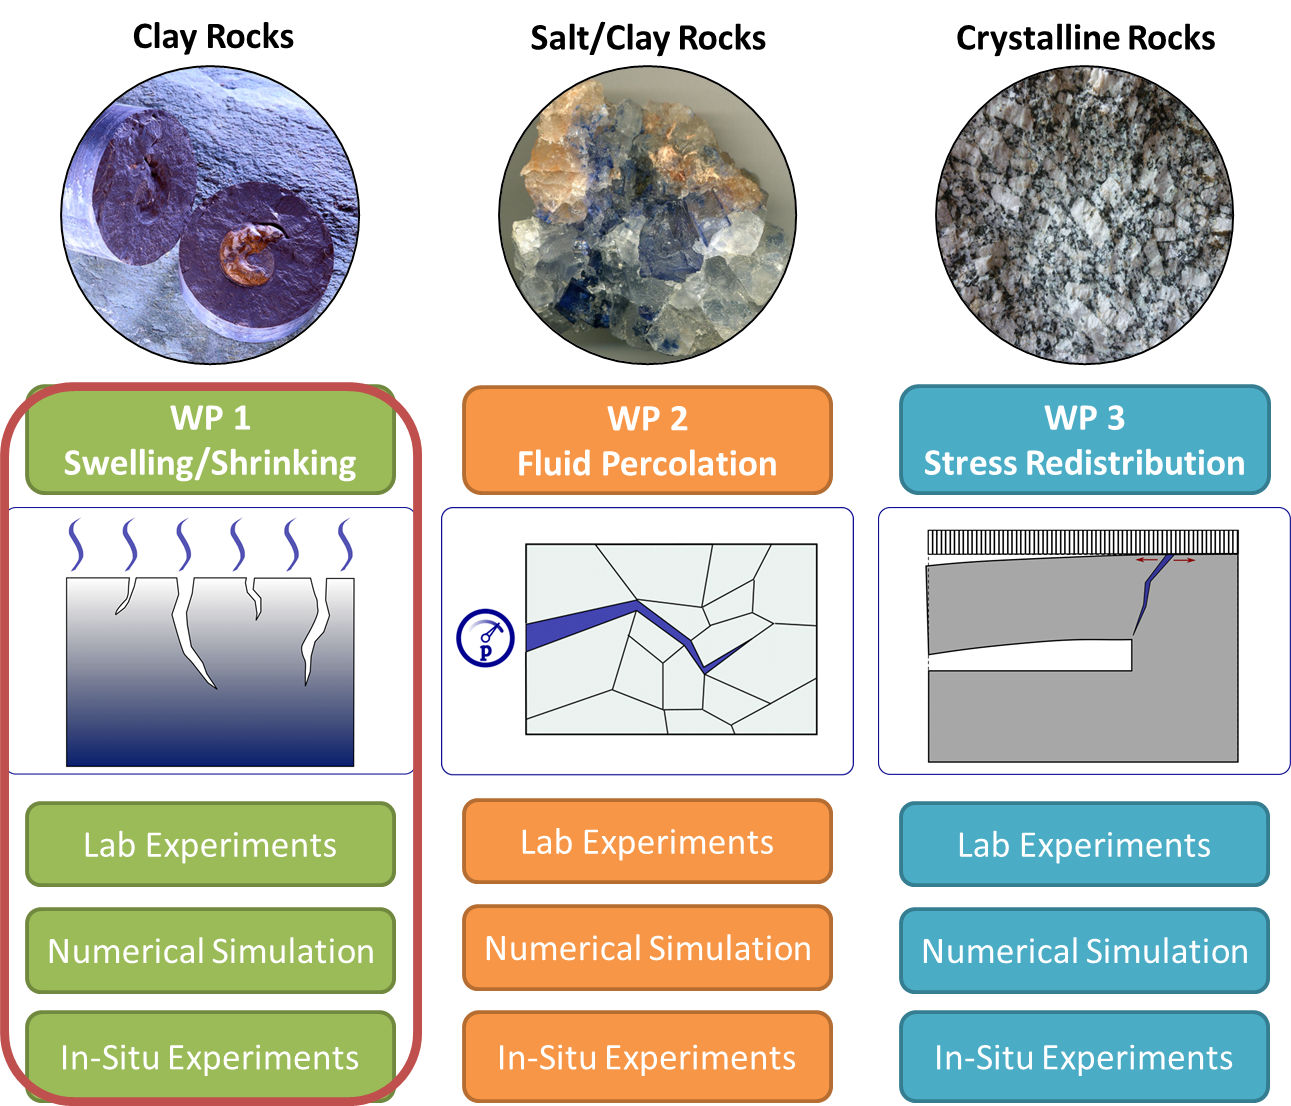
\includegraphics[width=1\textwidth]{figures/geomint-wp1a.png}
%\end{minipage}
%\hfill
%\begin{minipage}{0.49\textwidth}
%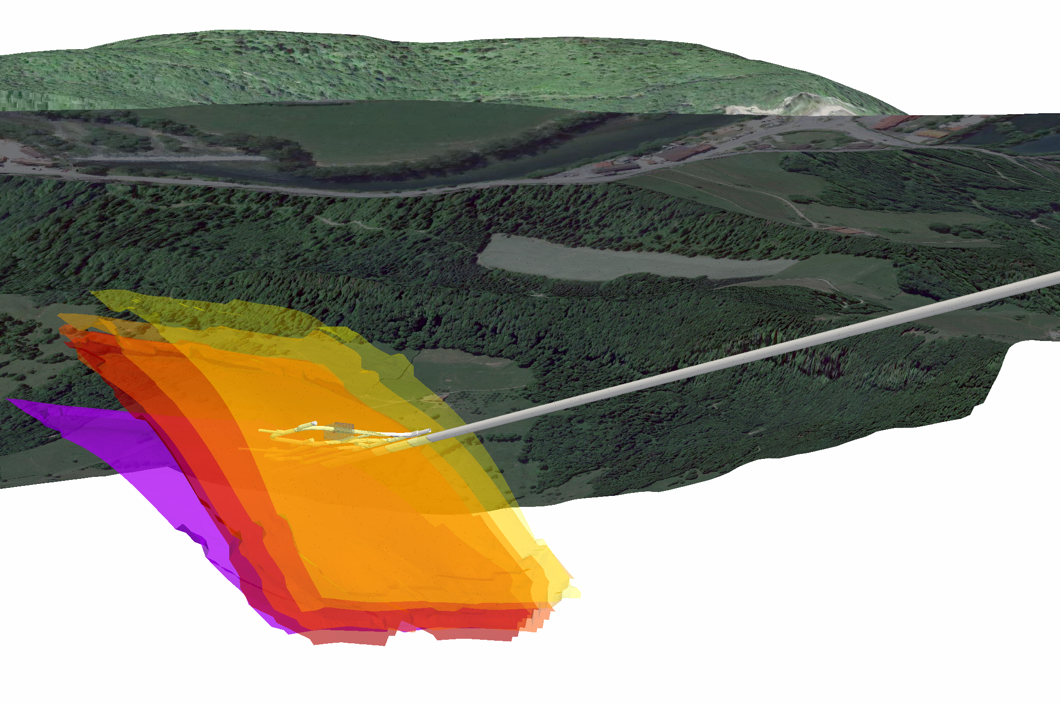
\includegraphics[width=1\textwidth]{figures/mt-vr-01.png}
%\end{minipage}
%\caption{Synthese in GeomInt: Verknüpfung prozessorientierter Arbeitspakete mit Virtual Reality (VR)-Methoden}
%\label{fig:pro03-de}
%\end{figure}

Die Projektergebnisse gestatten ein verbessertes Verständnis der Prozesse, der verwendeten Methoden und der anwendungsorientierten Systeme für relevante Zeit- und Längenskalen, um die Planung und Realisierung geotechnischer Nutzungen des Untergrundes sicherer, zuverlässiger und effizienter zu gestalten. Ein gewichtiger Vorteil von GeomInt ist die prinzipielle Übertragbarkeit der experimentell-numerischen Konzepte, Modelle und Methoden auf eine Vielzahl drängender wissenschaftlich-technischer Fragestellungen in den Geowissenschaften. Dies ermöglicht die Verwertung von Projektergebnissen für verschiedene politisch und gesellschaftlich relevante geotechnologische Nutzungen (z. B. tiefe Geothermie, Energiespeicherung, Endlagerproblematik, Methoden zur hydraulischen Stimulation, konventionelle und unkonventionelle Rohstoffgewinnung oder Tunnelbau). Diese Übertragbarkeit wurde insbesondere bei der methodischen Ausgestaltung des Vorhabens sowie bei der Dokumentation von Methoden, Ansätzen und Ergebnissen berücksichtigt und kann gleichzeitig als Grundlage für potenzielle Anschlussarbeiten zu GeomInt dienen.

\section*{Der GeomInt-Ansatz: lab, in-situ, in-silico, virtual reality}

Das GeomInt-Vorhaben basierte auf einer sehr engen Verknüpfung von experimentellen und numerischen Arbeiten. Drei Arbeitspakete konzentrierten sich auf verschiedene Mechanismen, welche die Barriereintegrität potenzieller Wirtsgesteine beeinflussen: (WP1) Quellen / Schrumpfen von Tongesteinen, (WP2) druckgetriebene Perkolation in Salz- und Tongesteinen sowie (WP3) Spannungsumlagerungen in kristallinen Gesteinen.
%
Abb.~\ref{fig:appraoch} zeigt die geografischen WP-Workflows von der In-situ Probenahme über die geomechanischen Laboratorien bis hin zur Modellierung. Die Hauptquellen für Gesteinsproben waren (i) Mont Terri für Tongestein, (ii) Springen für Salz und (iii) Freiberg / Kirchberg für kristalline Gesteinsproben. Darüber hinaus besteht eine Zusammenarbeit mit anderen URLs (Bure, Grimsel) in Bezug auf experimentelle und Modellierungsarbeiten – hauptsächlich zum Testen der Übertragbarkeit der Methodiken auf andere Gesteinsarten (z. B. Callovo-Oxfordian Clay - COx).

%\begin{figure}[ht!]
%\centering
%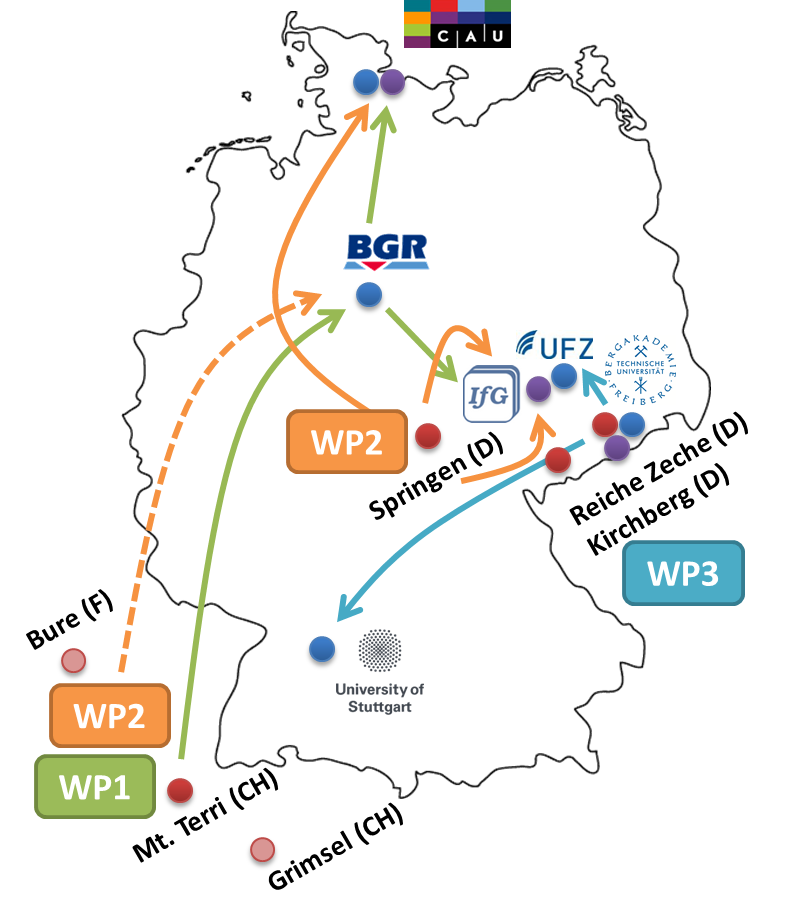
\includegraphics[width=0.7\textwidth]{figures/geomint-all.png}
%\caption{Geografischer Arbeitsablauf einschließlich miteinander verbundener experimenteller und Modellierungsarbeiten in GeomInt}
%\label{fig:appraoch-de}
%\end{figure}

Im Folgenden stellen wir den ''geographischen Workflow'' für die einzelnen Arbeitspakete kurz vor. Bitte beachten Sie, dass die Versuchs- und Modellierungsplattformen für die Analyse von Diskontinuitäten unabhängig von bestimmten Gesteinsarten eingerichtet wurden.

%\begin{figure}[ht!]
%\begin{minipage}{0.48\textwidth}
%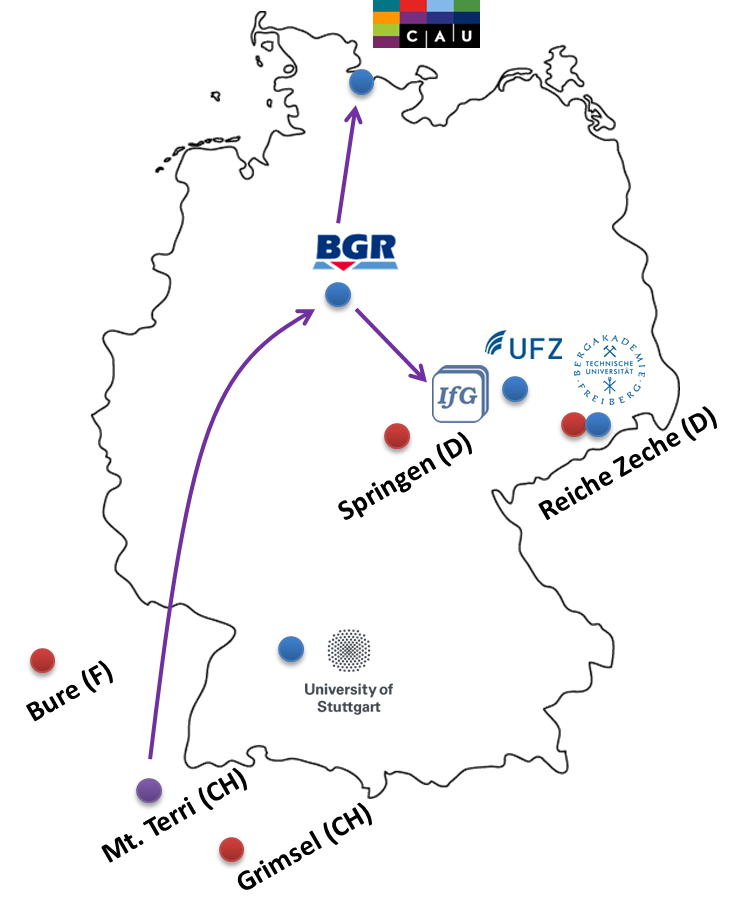
\includegraphics[width=\textwidth]{figures/geomint-wp1.png}
%\caption{WP1: Quellen / Schrumpfen}
%\end{minipage}
%\hfill
%\begin{minipage}{0.48\textwidth}
WP1 befasste sich mit Quell- und Schrumpfprozessen in Tonstein. Die BGR beschaffte \textbf{Opalinus Ton} Proben aus dem Untertagelabor Mont Terri (Underground Research Lab - URL) in der Schweiz und stellte sie den Partnern CAU und IfG in Kiel bzw. Leipzig für Laboruntersuchungen zur Verfügung. Die Proben stammten aus verschiedenen Ton- und Sandfazies. Die experimentelle Arbeit mit Proben aus der sandigen Fazies war wegen der gro{\ss}en Heterogenität des Materials besonders anspruchsvoll. Das WP1 war und ist weiterhin eng mit dem Mont Terri Projekt in Zusammenarbeit mit swisstopo verbunden.
%\end{minipage}
%\end{figure}

%\begin{figure}[ht!]
%\begin{minipage}{0.48\textwidth}
Fluid-Perkolationsprozesse wurden sowohl in \textbf{Ton- und Salzgesteinen}, d.h. in duktilen Materialien, untersucht. Proben von Opalinuston stammten aus Untertagelabor Mt. Terri (siehe oben). Salzgesteinsproben wurden hauptsächlich vom Standort Springen in Thüringen gewonnen. Experimentelle Arbeiten zur Perkolation wurden in den Labors von IfG und CAU in Leipzig und Kiel durchgeführt. WP2 untersuchte die Mechanismen der Perkolationsschwelle für beide Gesteinsarten in Abhängigkeit von hydro-mechanischen (HM) Prozessen (d.h. Fluiddruck und mechanisches Spannungsfeld).
%\end{minipage}
%\hfill
%\begin{minipage}{0.48\textwidth}
%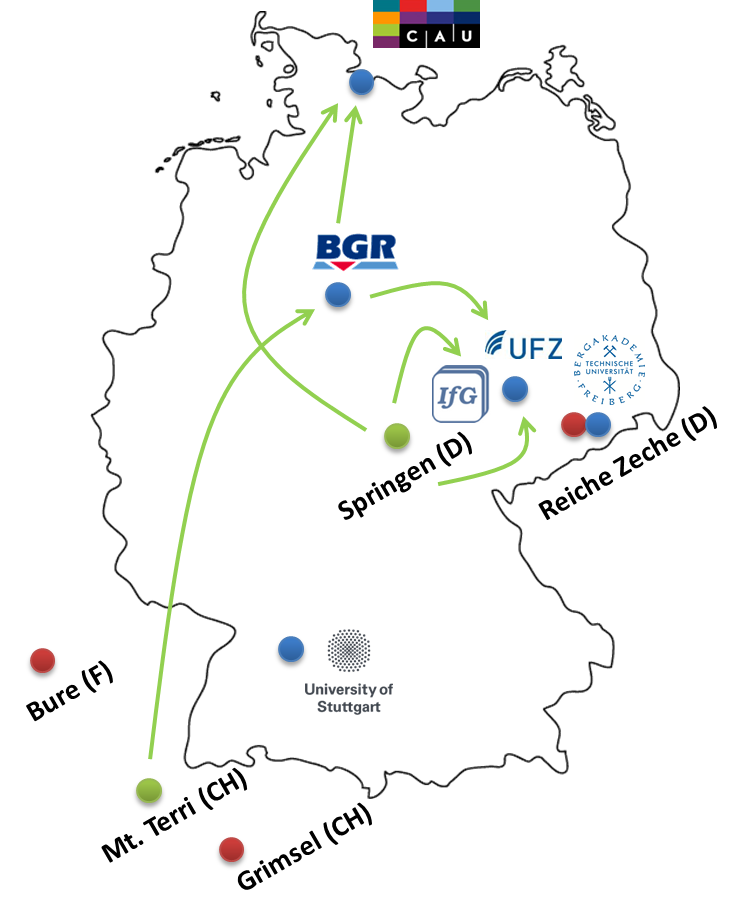
\includegraphics[width=\textwidth]{figures/geomint-wp2.png}
%\caption{WP2: Fluid-Perkolation}
%\end{minipage}
%\end{figure}

%\begin{figure}[ht!]
%\begin{minipage}{0.48\textwidth}
%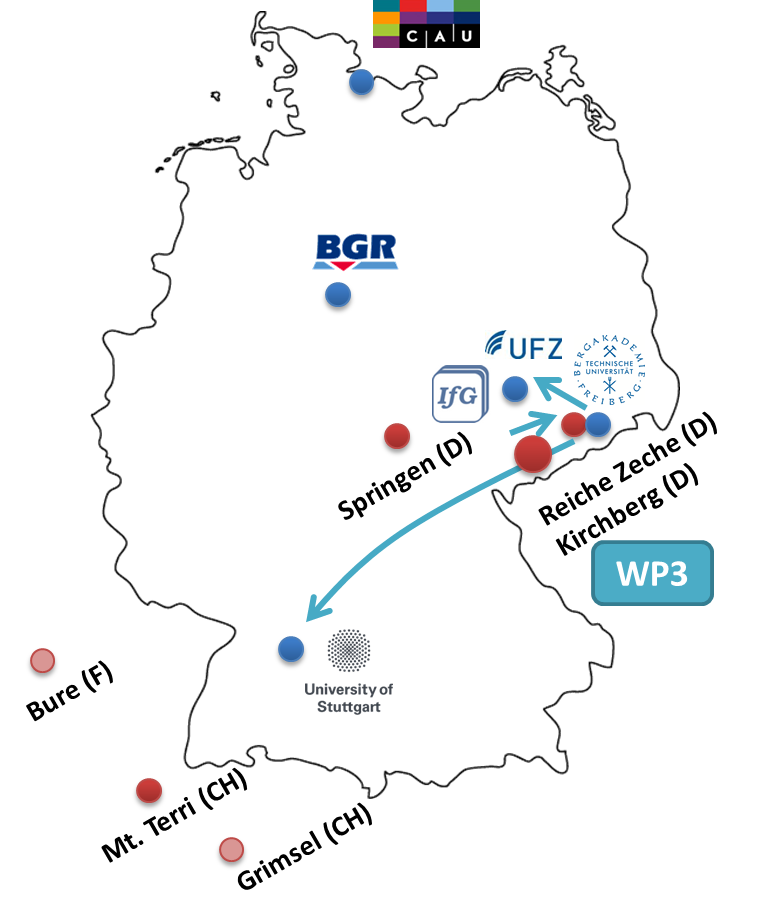
\includegraphics[width=\textwidth]{figures/geomint-wp3.png}
%\caption{WP3: Spannungsumlagerungen}
%\end{minipage}
%\hfill
%\begin{minipage}{0.48\textwidth}
WP3 untersuchte Diskontinuitäten, die durch Spannungsumlagerung in spröden Materialien entstehen. \textbf{Granitgestein} Proben wurden von Standorten im Erzgebirge, d.h. von Kirchberg und Freiberg, gewonnen (URL Reiche Zeche). Experimentelle Untersuchungen wurden in den Labors in Freiberg (TU Freiberg) und Stuttgart (Universität Stuttgart) durchgeführt. Es wurden Experimente mit konstanter Normallast (CNL) und konstanter Normalsteifigkeit (CNS) durchgeführt, um die Flüssigkeitsströmung in groben Brüchen unter einschränkenden Spannungen zu untersuchen. Gesteinsproben aus Freiberg werden auch beim ''Crystalline Task'' der neuen Phase DECOVALEX-2023 verwendet.
%\end{minipage}
%\end{figure}

Die Arbeiten der folgenden Forschungsinfrastrukturen wurden miteinander kombiniert:
\begin{itemize}
    \item \textbf{Gesteinsmechanische Labors}
	\begin{itemize}
		\item THM-gekoppelte Prüfung unter kontrollierten Randbedingungen
		\item Material- und Prozesscharakterisierung
	\end{itemize}
	\item \textbf{Numerische Methoden und Software}
	\begin{itemize}
		\item OpenGeoSys (XFEM, PFM)
		\item md-LEM (LEM)
		\item pythonSPH (SPH)
		\item UDEC, 3DEC (DEM)
		\item FLAC3D (FDM)
	\end{itemize}
	\item \textbf{Untertagelabore}
	\begin{itemize}
		\item Springen (Steinsalz, Kali)
		\item Mont Terri (Tongestein)
		\item Reiche Zeche (kristallines Gestein)
	\end{itemize}
	\item \textbf{Simulations- und Entwicklungsinfrastruktur}
	\begin{itemize}
		\item HPC-Cluster
		\item Versionsmanagement
		\item VISLAB (\url{www.ufz.de/vislab})
	\end{itemize}
\end{itemize}

%\begin{figure}[ht!]
%\centering
%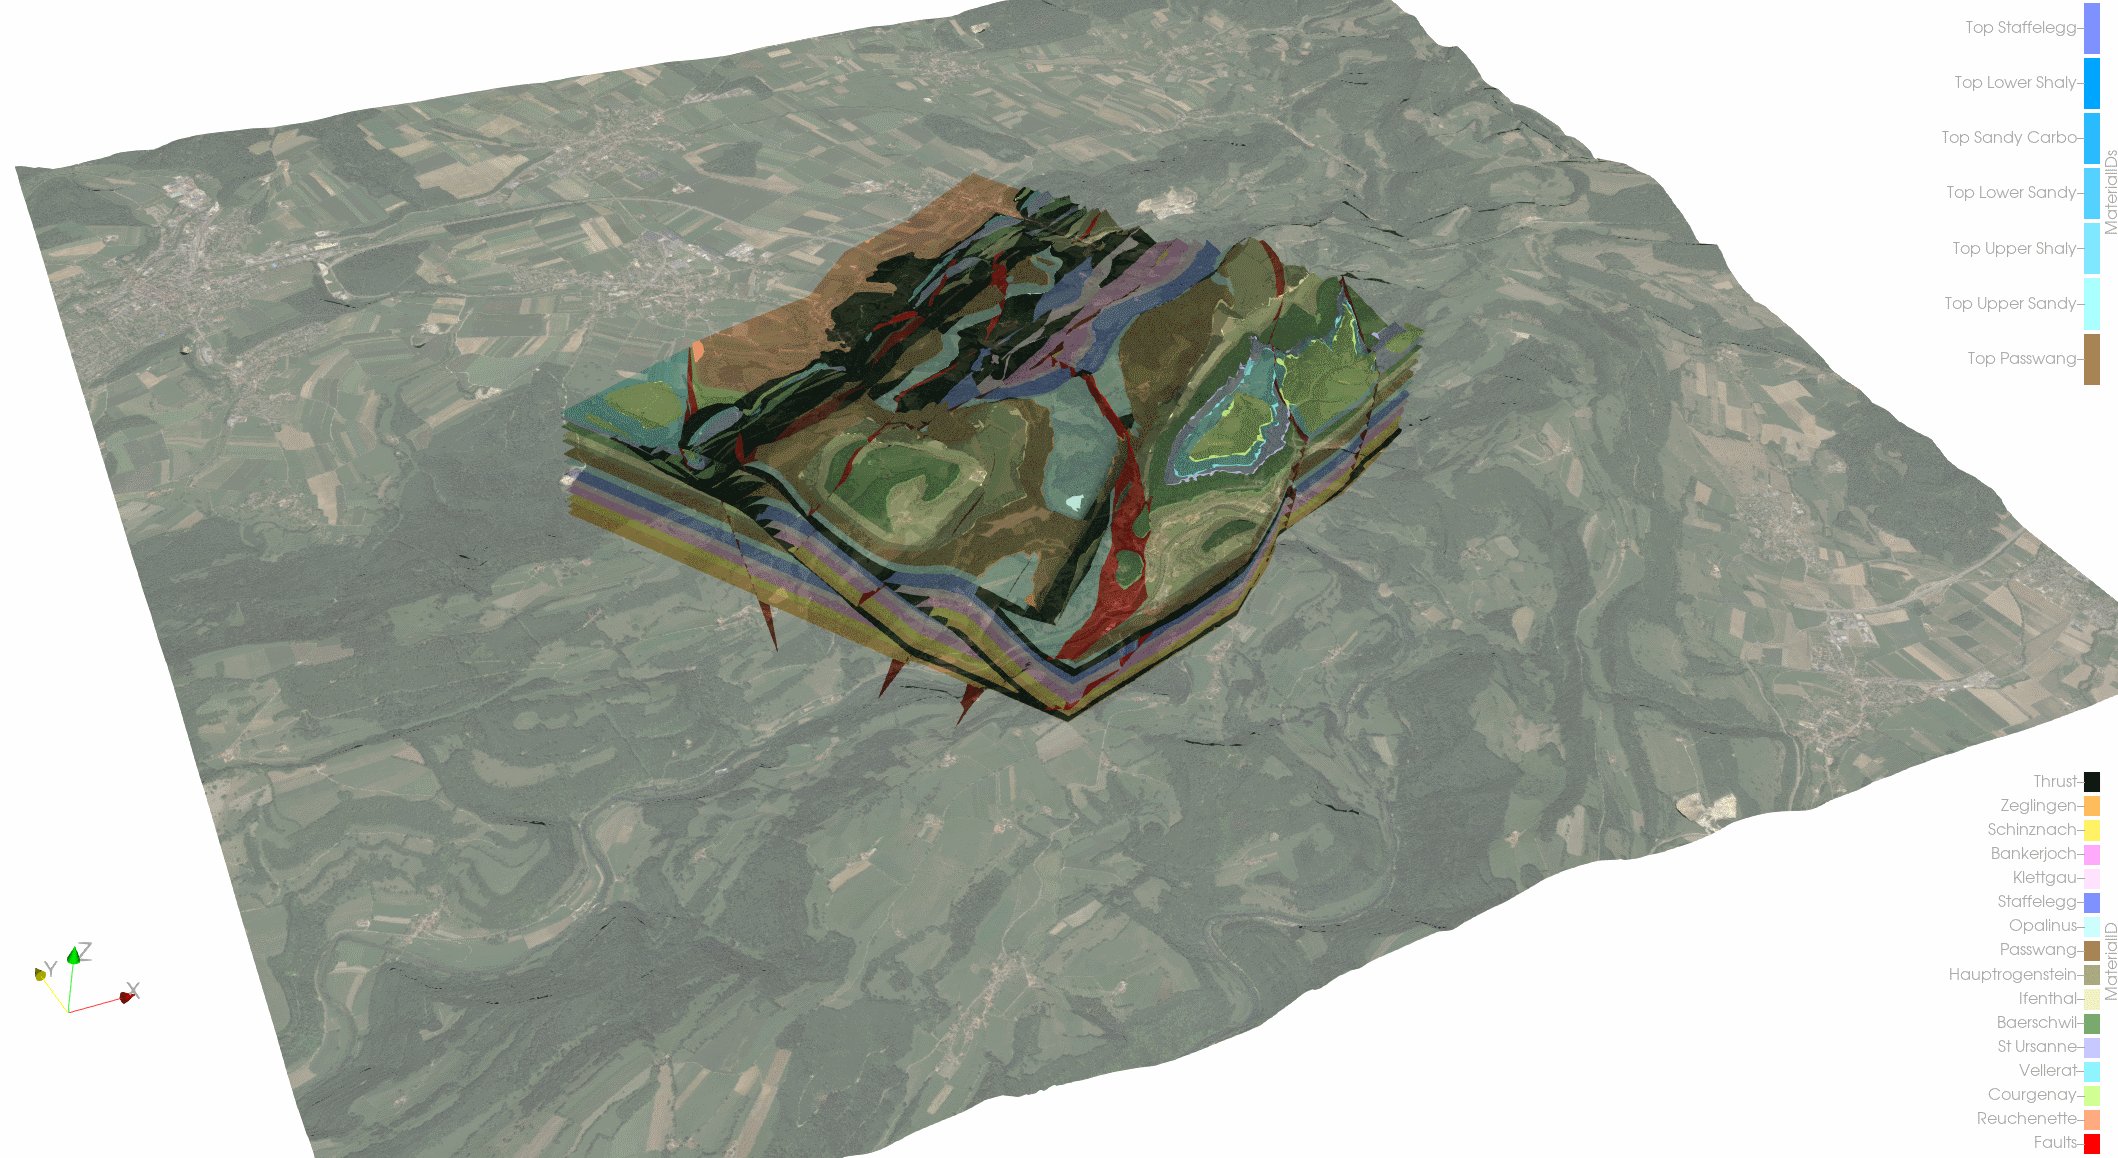
\includegraphics[width=0.9\textwidth]{figures/mt-surface+move.png}
%\caption{Virtuelles Untertagelabor Mont Terri: Virtuelle Daten- und Modellintegration in einem präzisen georeferenzierten Kontext (Karsten Rink)}
%\label{fig:vr-url-de}
%\end{figure}

Zusätzlich zu experimentellen (Labor und in-situ) und Modellierungsarbeiten verwendeten wir Methoden der Virtuellen Realität (VR) zur Daten- und Modellintegration sowie zur Visualisierung. Abb. \ref{fig:vr-url} zeigt eine Momentaufnahme des Virtual-URL-Projekts für Mont Terri. Die Grundidee besteht darin, alle Informationen aus In-situ- (und sogar Labor-) Experimenten sowie die entsprechenden Modelle in einem Virtual-Reality-Kontext - wie in einer visuellen Datenbank - zusammenzuführen. Auf die in VR eingebetteten Daten kann interaktiv und interoperabel zugegriffen werden \cite{Rink2020}.